\chapter{機能}\label{cha:Function}

本章では、本研究で試作したモータ特性表自動生成ツールの機能について説明する。\\

モータ特性表自動生成ツールは、OpenModelicaで、Modelica言語にて作成したモータの
モデルを、シミュレーションした時に出力されるcsvファイルを読み込み、実行することによって、モータ特性表を生成する。\\

\section{対応するモデル}\label{taioumodel}
試作したモータ特性表自動生成ツールでは、以下のModelicaモデルのシミュレーション結果に対応する。
\begin{itemize}
	\item モータ単体のModelicaモデル
	\item モータ単体のModelicaモデルをサブシステムとするモデル
\end{itemize}
なお、今回はモータの中でもブラシ付きDCモータに対応する。\\
以降、上記のモデルについて具体的に説明する。

\subsection{モータ単体のModelicaモデル}\label{sec:sub1}
モータ単体のModelicaモデルとは、電源部品、抵抗部品、インダクター部品、起電力部品、慣性部品、接地部品を
持つモデルのことである。\\
上記6つの部品が必要な理由は、ブラシ付きDCモータの等価回路\cite{等価回路}をModelica言語で表す際に
使用する部品\cite{modelicaシステム本}だからである。\\
ブラシ付きDCモータの等価回路を図\ref{fig:touka}に、モータ単体のModelicaモデルを図\ref{fig:tantai_model}に、
モータ単体のModelicaモデルをModelicaコードで表したものを図\ref{fig:tantai_modelica}に示す。

\begin{figure}[t]
	\centering
	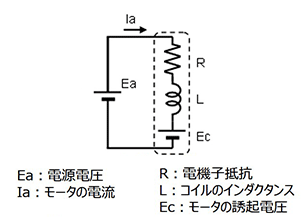
\includegraphics[width=10cm]{./Image/touka.png}
	\caption{等価回路}
	\label{fig:touka}
  \end{figure}

\begin{figure}[t]
  \centering
  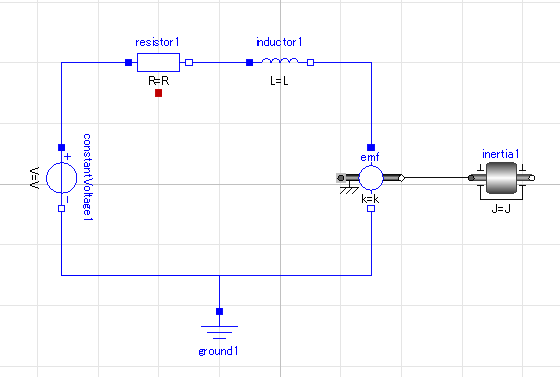
\includegraphics[width=10cm]{./Image/tantai_model.png}
  \caption{モータ単体のModelicaモデル}
  \label{fig:tantai_model}
\end{figure}

\begin{figure}[t]
	\centering
	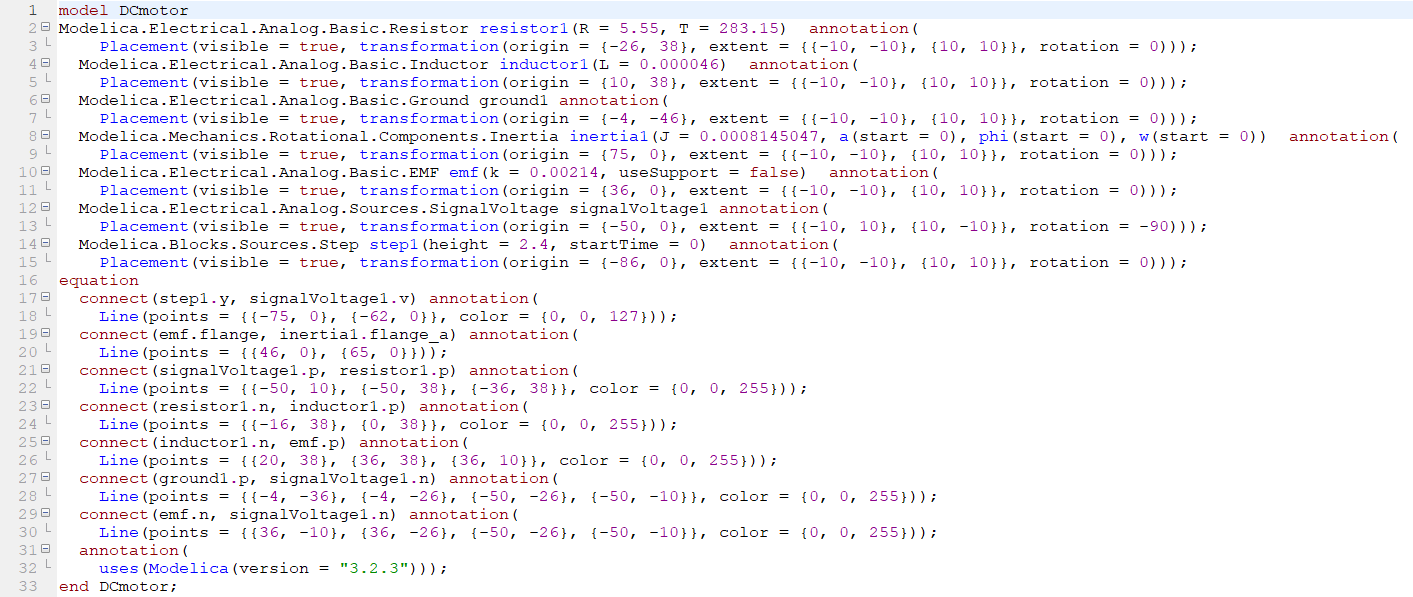
\includegraphics[width=16.5cm,height=8cm]{./Image/tantai_modelica.png}
	\caption{モータ単体のModelicaモデルのModelicaコード}
	\label{fig:tantai_modelica}
  \end{figure}

\subsection{モータ単体のModelicaモデルをサブシステムとするモデル}\label{sec:sub2}
モータ単体のModelicaモデルをサブシステム\cite{modelicaシステム本}(準備に書く?)とするモデルとは、\ref{sec:sub1}節で説明した
モータ単体のModelicaモデルを一つのモデルにして、サブシステムとして書いたモデルのことである。\\
例を図\ref{fig:subsisu_modelica}に示す。

\begin{figure}[t]
	\centering
	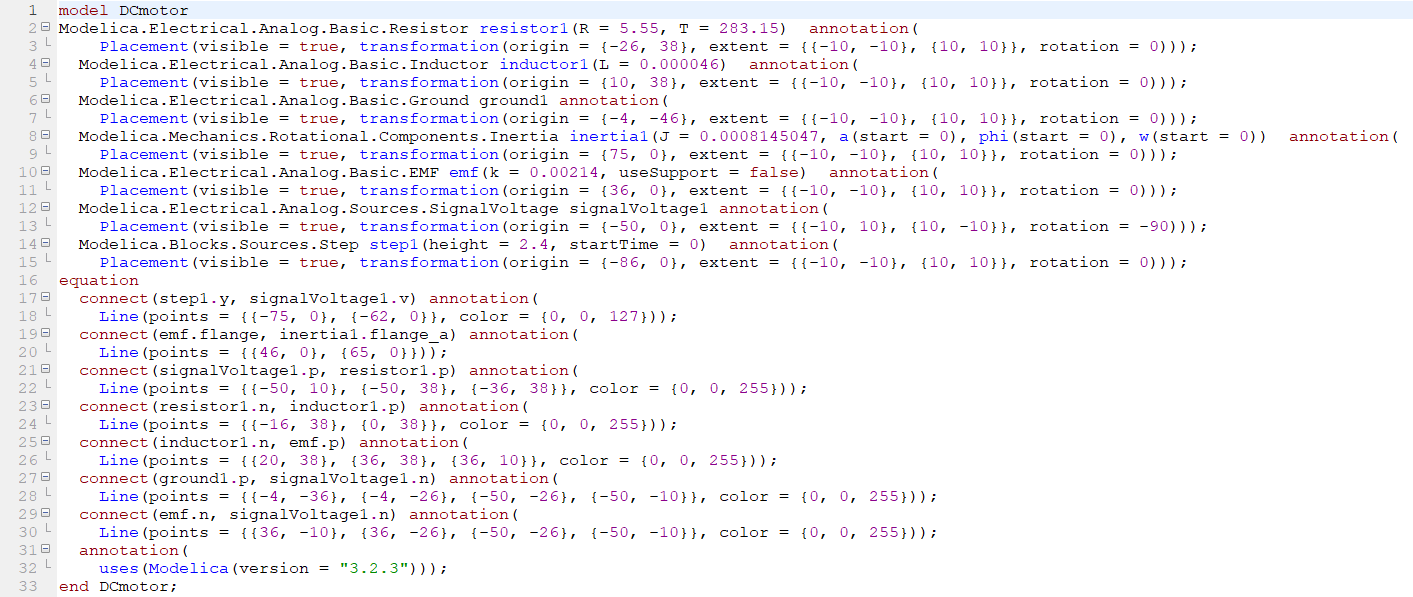
\includegraphics[width=16.5cm,height=8cm]{./Image/tantai_modelica.png}
	\caption{モータ単体のModelicaモデルをサブシステムとするモデル}
	\label{fig:subsisu_modelica}
  \end{figure}


\section{モータ特性表生成}\label{kenkyu_mokuteki}
今回試作したモータ特性表自動生成ツールは次の9個の要素を持つモータ特性表を生成する。

\begin{itemize}
	\item 電圧
	\item 始動電流
	\item 停動トルク
	\item 最大効率
	\item 定格トルク
	\item 定格回転数
	\item 定格電流
	\item 定格出力
	\item 最大回転数 
\end{itemize}

